\begin{figure*}[t]
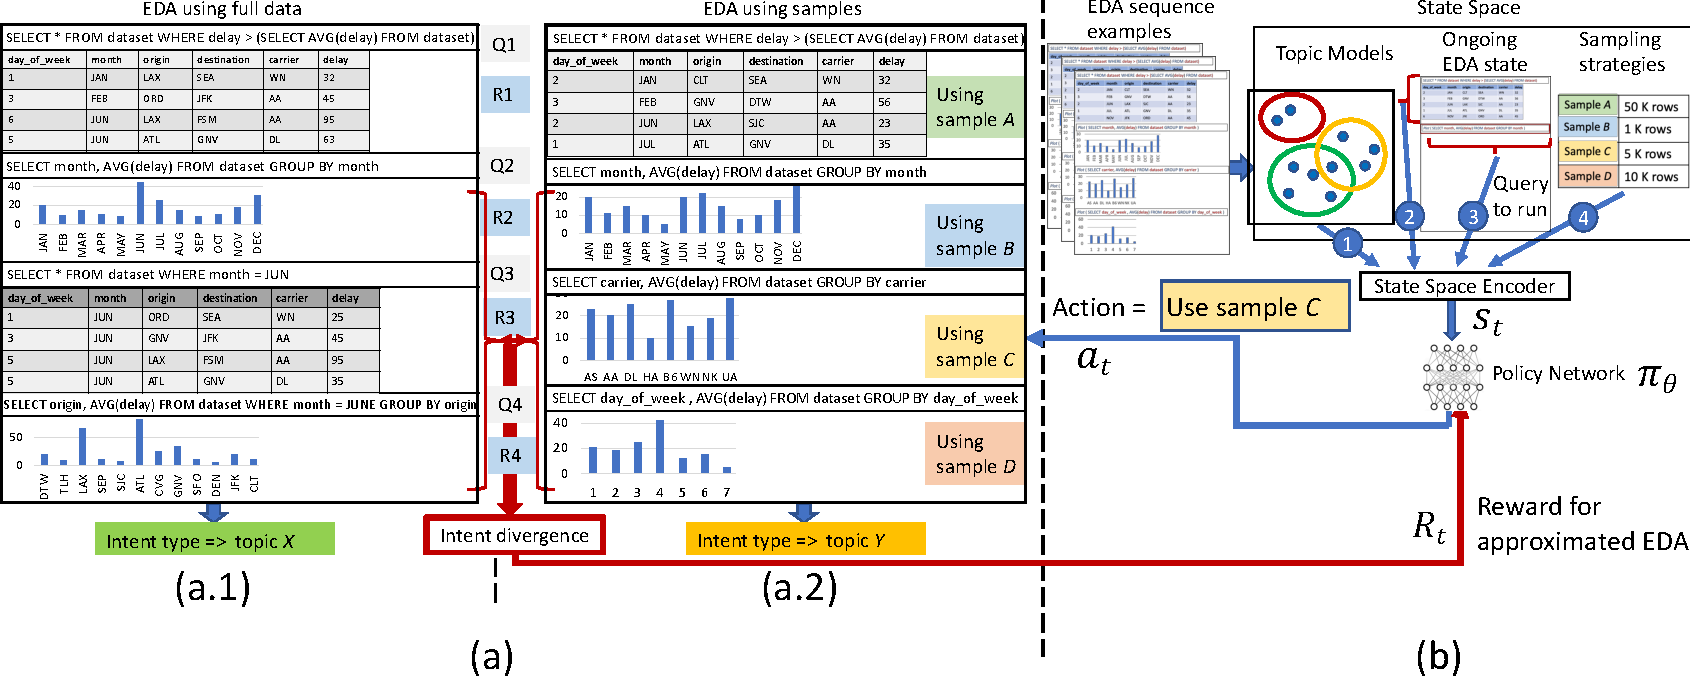
\includegraphics[width=0.98\linewidth]{LaTeX/figures/workflow.pdf}
     \caption{\textbf{(a)} Example of intent divergence between EDA sessions using full data \textbf{(a.1)} vs. using samples \textbf{(a.2)}. 
     Bad sample selection in (a.2) led to large errors in the result \textit{R2}. Consequently, user diverted from ideal query sequence and finally found misleading insight in \textit{R4}.
     \textbf{(b)} Workflow of our RL-based \name is shown. The agent transparently interacts with a live EDA session (e.g. one on the left) and chooses the best action $a_t$, i.e. the optimal sample to use for the current so that intent divergence is minimized. \name's \textit{State Space Encoder} combines 4 different information into a state $s_t$ that is used by the policy-network ($\pi_{\theta}$) to decide the best action. 
     %\tong{it seems that some content is cut in the right part of the figure 2 (b) (the state space seems to be a rectangle but the line on the very right part is missing).}
     }
     \label{fig:intent_divergence}
\vspace{-0.8em}
\end{figure*}



\section{Background and Motivations}
\begin{comment}
Exploratory data analyses (EDA) is an interactive process for insight generation for new datasets~\cite{milo2020automating, khan2020weblens, milo2018next} and low latency is important~\cite{liu2014effects},
%Several recent papers~\cite{kery2018story, rule2018exploration} present studies highlighting how computational notebooks combine code, visualizations, and text in a single document are increasingly being used by data analysts from different domains. 
%
%EDA being an interactive environment, low latency is key~\cite{liu2014effects}, and we envision that similar to the way sampling is used to speed up ad-hoc query processing in databases~\cite{park2018verdictdb}, it can also be used for EDA to run corresponding queries on samples at the back-end\cite{galakatos2017revisiting}.
%
However, EDA being a highly sequential decision making process by the data-analysts with some \textit{non-explicit intentions} in their minds, poor choice of sampling strategy in an attempt to reduce interaction latency, can completely diverge the exploration process and lead to unsuccessful EDA sessions or misleading insights.
%
\end{comment}

\subsection{Motivating Example}

%\noindent \textbf{Motivating example:}

In Figure~\ref{fig:intent_divergence}(a.1), we show example of an EDA being performed on \textit{all} the records of Flights data~\cite{Flights}. At first an analyst attempts to understand the flights delay and filters the entries that had delay higher than average (with query \texttt{Q1} and corresponding result/visualization \texttt{R1}). 
Then she wants to understand delays in detail by grouping those by \textit{month} (i.e. \texttt{Q2}) and observes from the bar-plot (\texttt{R2}) that month of \texttt{JUN} contributed highest delays.
Then she inspects by filtering the rows only for \texttt{JUN} (\texttt{Q3} and \texttt{R3}). Not finding anything obvious she groups these filtered results by \texttt{origin} airport (\texttt{Q4}) and from the result (\texttt{R4}) concludes that delays in flights originating from \texttt{LAX} and \texttt{ATL} airports is the main culprit. Then she might forward this \textit{insight} and investigate the root-cause of delays in these airports further. 
Please note: there is a lack of explicit intents~\cite{milo2020automating, ma2021metainsight} from the analysts corresponding to an EDA session.
%as they interactively decide what to do next when they see the outcome of previous results~\cite{rule2018exploration}.

Now in Figure~\ref{fig:intent_divergence}(a.2), we illustrate the problem of arbitrary sample selection if sampled are used to speed-up queries but with approximate results.
While nothing detrimental happens in the result \texttt{R1} and the analyst would still run (\texttt{Q2}) to understand the delays grouped by \texttt{month}, a poor choice of sample may not highlight the large amount of delay contributed by the month of
\texttt{JUN}. 
Therefore, not finding anything that stands out over different months, the analyst might go on to look for other anomalies or patterns of delay for different careers (\texttt{Q3} and \texttt{R3}) and further not finding anything that suspicious, attempts to understand delays over different \texttt{days\_of\_week}(\texttt{Q4} and \texttt{R4}) and concludes with a \textit{misleading insight} that delays are primarily caused of flights on \textit{$4^{th}$ day of the week}.
%
Here the analyst diverged from the ideal analysis flow (if original data was used) because of approximation errors in queries/results \texttt{Q1/R1} and \texttt{Q2/R2}. 
She finally made a wrong decisions on her choice of subsequent queries at \texttt{Q3}.   
As a result overall EDA flow diverged. 
%%Such intent-divergence can be avoided and still speed of interactions can be optimized through sampling by a more intelligent EDA-system. 

%I\noindent\textbf{Takeaway:} 
Considering the above example, appropriate sub-sample selection is crucial based on the context of EDA at each step. Thus balancing low latency for good interactive experience vs. intent and insight preservation is the goal of this paper. 
%\sm{“The authors introduce a new concept of intent-divergence early on (ln 164), but however, never explain it in any detail. It remains unclear why the proposition prevents an intent-divergence of the user. If the analyst’s intent actually changes, preventing an intent divergence on the model side, seems to hinder their workflow.The manuscript does not include a discussion of the relevant problem of “intent-shift”.”}


\subsection{Sampling Strategies}

A sample dataset $T_s$ is a subset of rows from an original dataset $T$. Following different sampling strategies select these subsets differently with different set of parameters that control the size and statistics of $T_s$.
We consider sampling strategies listed in Table~\ref{tab:actions} with different associated parameters that control the sizes of the subsamples and consequently the amount of statistical information. More details of the sampling strategies is in Appendix \textbf{\ref{app:sampling_details}}.

\begin{table}
\scalebox{0.8}{
 \begin{tabular}[ht!]{|l|l|l|}
    \hline
    {Sample Name} & {Short Name} & {Parameters} \\
    \hline
    {Uniform} & {Uni@$\tau$} & {$\tau$= [0.01, 0.05, 0.1]} \\
    \hline
    {Systematic} & {Sys@$k$} & {$k$= [100, 20, 10]}  \\
    \hline
    {Proportional stratified} & {Strat@$\tau$} & {$\tau$= [0.01, 0.05, 0.1]} \\
    \hline
    {At most $K$ stratified} & {Strat-K@$K$} & {$K$= [2k, 10k, 20k]} \\
    \hline
    {Cluster} & {Clus@$k$} & {$k$= 10, $\tau$= [0.01, 0.05, 0.1]} \\
    \hline
    {MaxMin Diversity} & {MaxMin@$k$} & {$k$= 0.1*$|T|$} \\
    \hline
    {MaxSum Diversity} & {MaxSum@$k$} & {$k$= 0.1*$|T|$} \\
    \hline
    \end{tabular}
    }
 \captionof{table}{Sampling strategies and corresponding parameters that together creates our action space. We use the \textit{Short Name} to refer these.}
 \label{tab:actions}
\end{table}

%We now provide brief background for different sampling strategies we used. 


\begin{comment}
    \item 
    \textbf{MaxMin Diversity:} 
    This maximises the minimum pairwise diversity between elements of $T_s$,
    %We define the $div$ function as follows,
    %
    %$div(T_s') = \underset{i,j \in T_s', i \neq j}{\mathrm{min}}\, d(i,j) $
    
    \item 
    \textbf{MaxSum Diversity:}
    This maximises the average pairwise diversity between elements of $T_s$. 
    %We define the $div$ function as follows,
    %
    %$div(T_s') = \frac{1}{|T_s|}\underset{i,j \in T_s', i \neq j}{\mathrm{\sum}}\, d(i,j) $
\end{comment}

\begin{comment}
\subsection{Reinforcement Learning}

In RL, at a high-level, an agent interacts with a system and tries to learn an optimized policy.
At each time step $t$, the agent observes the \textit{state} of the system $s_t$, and chooses to take an \textit{action} $a_t$ that changes the state to $s_{t+1}$ at time step $t+1$, and the agent receives a reward $r_t$.
The goal of the agent is to learn the
best policy to maximize its
expected cumulative discounted reward: $E[\sum_{t=0}^{\infty}\gamma^{t}r_t]$ where $\gamma \in (0,1)$ determines how much the future rewards contribute to the total reward~\cite{sutton1998reinforcement}.
In DRL, neural networks are used as agents to handle large state and action spaces~\cite{lillicrap2015, mnih2015human}. We explored few different RL algorithms and found that policy-gradient-based Advantage Actor Critic (A2C)~\cite{} with the neural network as a function approximator works best for our problem setup.
\end{comment}